\section{Simulation}\label{sec:simulation}
\frame{\tableofcontents[currentsection]}

%-------------------------------------------------
\subsection{Simulation Elements}\label{subsec:simulation-elements}

\begin{frame}
    \frametitle{Simulation Elements}
    The aim of the simulation is to determine whether a situated recommendation system may help reduce the waiting time needed to benefit from an attraction.

    \bigskip

    In order to achieve this, two simulations will be developed:
    \begin{enumerate}
        \item \textbf{Random Redirection} reflecting the current system.
        \item \textbf{Recommended Redirection} reflecting the desired system.
    \end{enumerate}

\end{frame}
%------------------------------------------------

\subsection{The Simulator}\label{subsec:the-simulator}

\begin{frame}
    \frametitle{The Simulator}
    As for the implementation of the simulation, the \textit{Alchemist Simulator} was used for many reasons:
    \begin{itemize}
        \item It provides a \textit{ready-to-use} simulation environment.
        \item It provides an intuitive graphic user interface.
        \item To contribute to the \textit{research and development} area of the \textit{UniBo DISI}.
    \end{itemize}

    \bigskip

    \begin{center}
        \includegraphics[width=0.5\textwidth]{../img/model}
        \label{fig:model}
    \end{center}

\end{frame}
%------------------------------------------------

\subsection{The Environment}\label{subsec:the-environment}

\begin{frame}
    \frametitle{The Environment}
    The map of Mirabilandia, along with its streets, is provided by \textit{OpenStreetMap}.

    \bigskip

    The deployed entities (Alchemist nodes) are \textbf{visitors} and \textbf{attractions}.
    Visitors are represented by black dots, while attractions are squares of different colors depending on their type (restaurant or ride).

    \bigskip

    Communication happens through attractions that are considered as \textbf{access points} that spread information to their neighbourhood.

\end{frame}

\begin{frame}
    \frametitle{The Environment}

    \begin{center}
        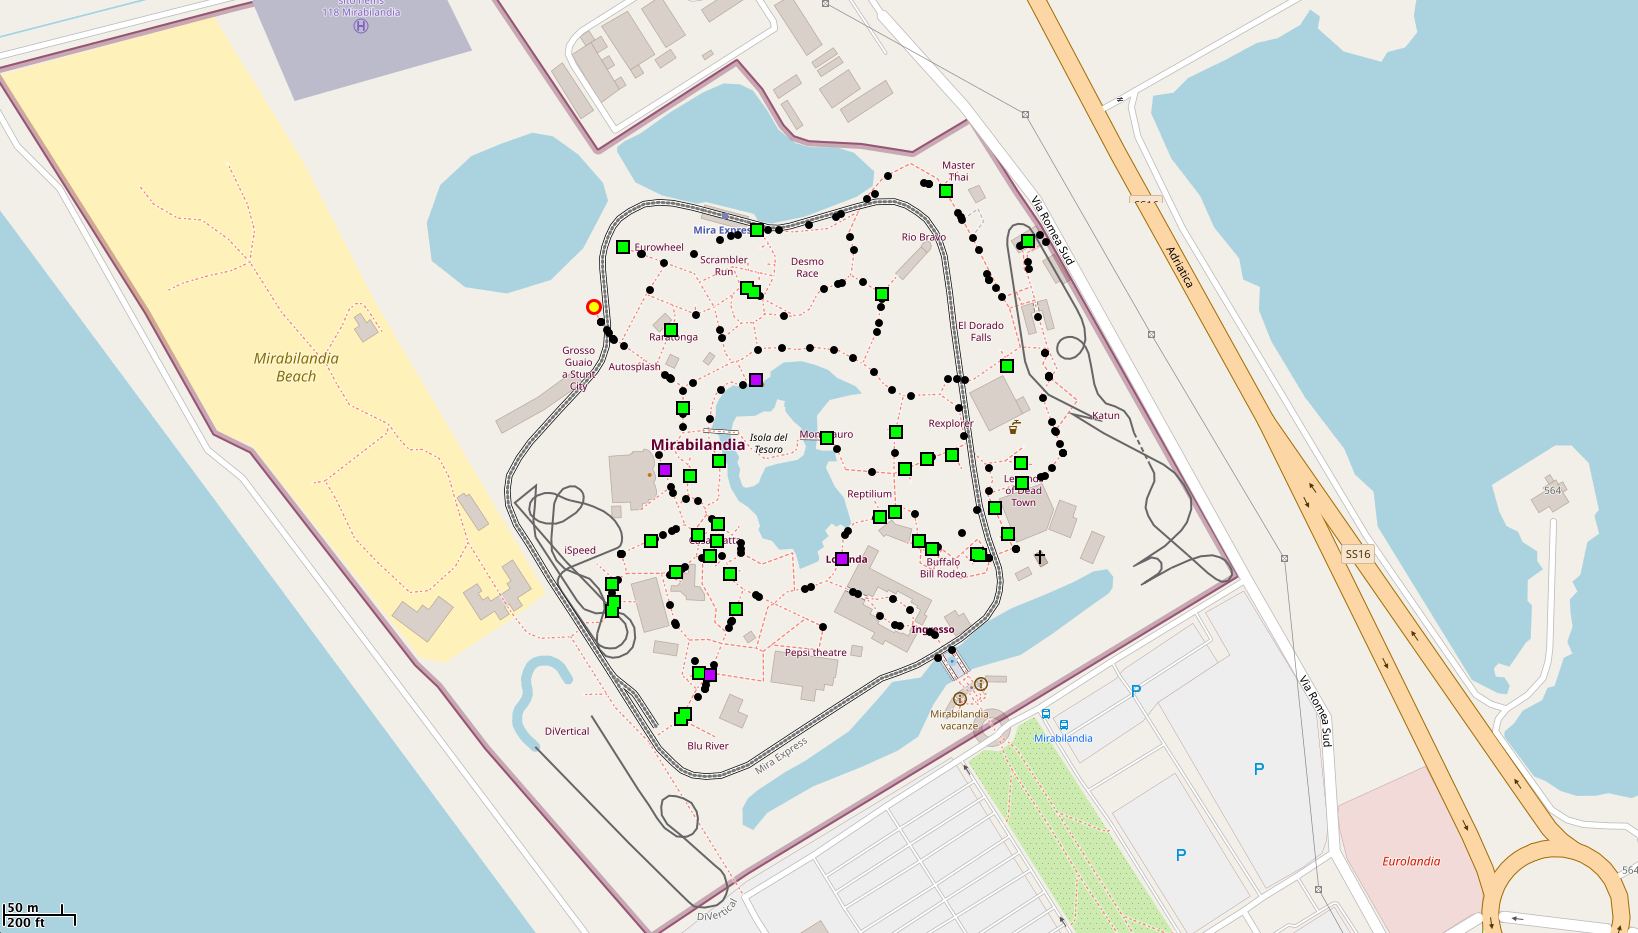
\includegraphics[width=0.9\textwidth]{../img/simulation-screenshot}
        \label{fig:simulation-screenshot}
    \end{center}

\end{frame}
%------------------------------------------------

\subsection{Redirection Policies}\label{subsec:redirection-policies}

\begin{frame}
    \frametitle{Redirection Policies}
    It is possible to define custom policies that allow determining the \textbf{next attraction} for a visitor.
    For the sake of the current simulations, the following policies were analyzed:
    \begin{itemize}
        \item \texttt{RandomPolicy}: performs a \textit{random redirection} by choosing one of the attractions inside the park randomly.
        \item \texttt{ShortestQueuePolicy}: performs a \textit{recommended redirection} by choosing the attraction with the shortest queue inside the whole park.
        \item \texttt{ShortestQueueInRangePolicy}: performs a \textit{recommended redirection} by choosing the attraction with the shortest queue within a given range with regard to the visitor.
    \end{itemize}

\end{frame}

\begin{frame}
    \frametitle{Redirection Policies}
    \begin{columns}
        \begin{column}{0.1\textwidth}
        \end{column}
        \begin{column}{0.3\textwidth}
            The two plots show the average waiting time per attraction with the described policies respectively with 500 and 3000 visitors.
        \end{column}
        \begin{column}{0.7\textwidth}
            \begin{center}
                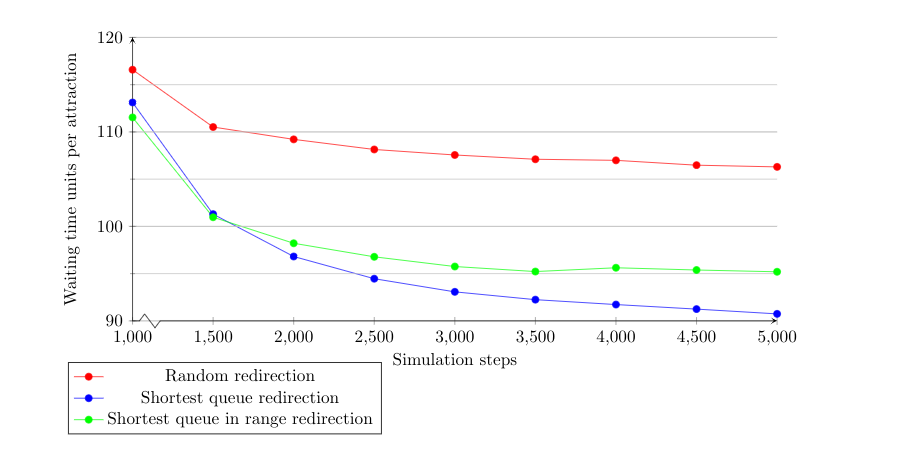
\includegraphics[width=0.8\textwidth]{../img/ratio-500}
                \label{fig:ratio-500}
            \end{center}
            \begin{center}
                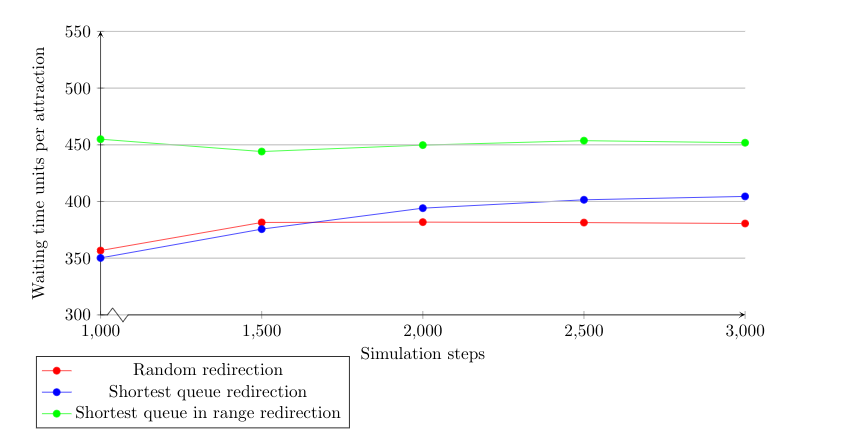
\includegraphics[width=0.8\textwidth]{../img/ratio-3000}
                \label{fig:ratio-3000}
            \end{center}
        \end{column}
    \end{columns}
\end{frame}

\begin{frame}
    \frametitle{Redirection Policies}
    Although the outcome of the simulation with 500 visitors went exactly as expected, it was not the case for the one with 3000 visitors.
    This could be caused by disparate reasons:
    \begin{itemize}
        \item The policies may be too simple.
        In fact, the attractions that in a given moment are less crowded end up being the most crowded a few moments later because a huge amount of visitors is redirected there.
        \item The simulation does not perfectly match the reality: not all the visitors in a real scenario will accept the recommendation received.
        Moreover, at the current state of the simulation visitors’ interests and preferences are not taken into account.
    \end{itemize}

\end{frame}

%------------------------------------------------

